\section{Empirical Test on EEG Measurements}
Consider now the same estimation of the number of active sources, $k$, but from the real EEG measurements. 
For this estimation one can not compare the estimation to the real sources as in the previous section.
Hence, the replica count method is just applied an estimation $\hat{\mathbf{X}}_{\text{main}}$ of real EEG measurements and a conclusion is made from the observed result.

The source signal estimation is performed on segment 10 from the S1\_Cclean EEG data set, where every second sensor is removed to achieve the case where $M<N$. 
Specifically $\hat{\mathbf{X}}_{\text{main}}$ is computed given $k=N$ and $\hat{\textbf{A}}_{fix}$ resulting from segment of EEG measurements specified by $M = 1/2N = 13$. 
%For the estimation one must give an initial guess for the number of active sources. 
%Remember that $k > M$ and $k < N$.  
%$k = 17$ has been chosen as a choice for how many active sources exists in time segment $s = 10$
\todo{hvad? det skal vel være k=N, lav ny figur uden y aksen og med title}. 

Figure \ref{fig:eeg_k} visualize the recovered source matrix $\hat{\mathbf{X}}_{\text{main}}$ from time segment $s = 10$ for $M = 13$ and $k = N = 27$.
\begin{figure}[H]
    \centering
	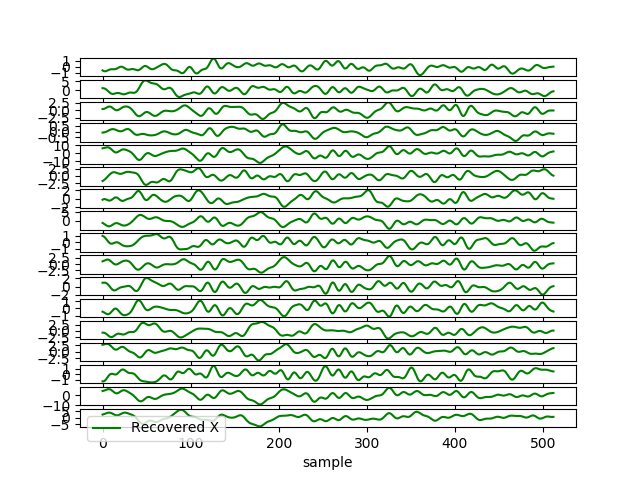
\includegraphics[scale=0.5]{figures/ch_estimate/eeg_k_timeseg_10.png}
	\caption{The recovered source matrix $\hat{\mathbf{X}}_{\text{main}}$ from time segment $s = 10$ from S1\_Cclean for $M = 13$ and $k = N = 27$.}
	\label{fig:eeg_k}
\end{figure}
\noindent
From figure \ref{fig:eeg_k} it is seen that all $N$ source signals appears to be active, furthermore there seem not to be any visible indication of an active source being non-active, with respect to being a direct replica. 

By applying the replica count method to $\hat{\mathbf{X}}_{\text{main}}$  from figure \ref{fig:eeg_k} only four sources are not considered replicas. 
These potentially active sources are found in row 2, 5, 16 and 17. 
This leads to the conclusion that for time segment $s = 10$ with system specification $M = 13$ for the S1\_Cclean EEG data set only have $k = 4$ active sources. 



